\chapter{Non-isothermal two-phase flow consolidation}
\label{sec:th2m}

%------------------------------------------------------------------------------
\section{Balance equations}

In section \ref{sec:thm} we considered non-isothermal flow in an unsaturated deformable porous medium using the Richards model.
In this section we treat the partially saturated porous media as multi-phase system composed of constitutes with
the voids of the solid skeleton filled with water and gas. Similar to what presented in \cite{SanPesSch:06}, we assume that
capillary pressure $p_c$, gas pressure $p^g$, temperature $T$, and solid displacement $\Disp$ are primary variables
to describe the state of the porous media. The general notation for the multi-phase, multi-componental formulation is
\begin{align}
\dens_k^\gamma
\end{align}
where
$k$ is component and $\gamma$ is phase identification.
The governing equations are given hereafter.

%------------------------------------------------------------------------------
\subsection{Non-isothermal two-phase flow}

For liquid water $\dens^l$, vapor $\dens_w^g$ and the solid skeleton $\dens^s$, the mass balance is governed by the following equation:
\begin{align}
\poro(&\dens^l-\dens_w^g)(\pD{\sat^l}{T}{\dot T}
+
\pD{\sat^l}{p_c}{\dot \pres}_c)
+
\poro(1-\sat^l)(\pD{\dens_w^g}{T}{\dot T}
+
\pD{\dens_w^g}{p_c}{\dot \pres}_c)
\nonumber\\
&+
[\dens^l\sat^l+(1-\sat^l)\dens_w^g]\nabla{\dot \Disp}
-
\nabla\left[\dens^g\dfrac{M_a M_w}{M_g^2}\mathbb{D}_w^g\nabla\left(\dfrac{\pres_w^g}{\pres^g}\right)\right]
\nonumber\\
&+
\nabla\left[\dens^l\dfrac{\per\RelKa^l}{\mu^l}\left(-\nabla \pres^g+\nabla \pres_c+\dens^l \grv \right)\right]
\nonumber\\
&+
\nabla\left[\dens_w^g\dfrac{\per\RelKa^g}{\mu^l}\left(-\nabla\pres^g+\dens^g\grv\right)\right]-\beta_T\dot T
=
0
\end{align}
While, for dry air and the solid skeleton, the mass balance equation is given by
\begin{align}
-
\poro&\dens_a^g(\pD{\sat^l}{T}{\dot T}
+
\pD{\sat^l}{p_c}{\dot \pres}_c)
+
(1-\poro)(1-\sat^l)\beta^s\dens_a^g{\dot T}
\nonumber\\
&\poro(1-\sat^l)(\pD{\dens_a^g}{T}{\dot T}
+
\pD{\dens_a^g}{p_c}{\dot \pres}_c
+
\pD{\dens_a^g}{p^g}{\dot \pres}^g)
\nonumber\\
&+
[\dens^l\sat^l+(1-\sat^w)\dens_a^g]\nabla{\dot \Disp}
\nonumber\\
&-
\nabla\left[\dens^g\dfrac{M_a M_w}{M_g^2}\mathbb{D}_a^g \nabla(\pD{\pres_a^g}{\pres^g})\right]
\nonumber\\
&+
\nabla\left[\dens_a^g \dfrac{\per\RelKa^g}{\mu^l}\left(-\nabla\pres^g+\dens^g\grv\right)\right]
=
0
\end{align}
where
$\dens^l$, $\dens_w^g$, $\dens_a^g$ are liquid, vapor, air density, respectively;
$\mu^l$, $\mu^g$ are liquid and gas viscosities, respectively;
$\sat^l = 1 -\sat^g$ is liquid saturation;
$M_w$, $M_a$, $M_g$ are water, air, and gas molar masses, respectively;
$\mathbb{D}_w^g$ is vapor diffusion coefficient;
$\per$, $\RelKa^l$, $\RelKa^g$ are saturated and relative permeabilities for liquid and gas phases, respectively;
$\grv$ is gravity acceleration vector and
$\beta_T = n\sat^l\beta^l + n\sat^g\beta^g + (1-n)\beta^s$ is thermal expansion coefficient of the porous medium.

%------------------------------------------------------------------------------
\subsection{Deformation}

The thermo-poro-elastic deformation process in the porous medium is described by the momentum balance in terms of stress equilibrium:
\begin{align}
\nabla\cdot
\left(
\sigma - \alpha_b \max(p^g-S^l p_c, 0) - \beta_T (T-T_0) \mathbf I
\right)
+ \rho \mathbf g
=
0
\end{align}
where
$\sigma$ is effective stress;
$\alpha_b$ is Biot coefficient;
$T_0$ is reference temperature and
$\mathbf I$ is identity tensor.

%------------------------------------------------------------------------------
\subsection{Heat transport}

Heat transport in two-phase flow including storage, advection, diffusion processes in porous medium consisting of liquid, gas, and solid phases is described by following equation
\begin{align}
c\rho \frac{\p T}{\p t} + (c\rho \mathbf v)^f \cdot \nabla T - \nabla (\kappa \nabla T) = Q_T
\end{align}
where
\begin{align}
c\rho &= nS^l c^l \rho^l + nS^g c^g \rho^g + (1-n) c^s \rho^s
\nonumber
\\
(c\rho \mathbf v)^f &= nS^l c^l \rho^l \mathbf v^l + nS^g c^g \rho^g \mathbf v^g
\\
\kappa &= nS^l \kappa^l + nS^g \kappa^g + (1-n) \kappa^s
\nonumber
\end{align}
are heat capacity, fluid phase part for heat advection, and thermal heat conductivity of the porous medium, respectively

%------------------------------------------------------------------------------
\section{Constitutive equations}
\subsection{Density}

Liquid density is affected by thermal expansion effects
\begin{align}
\dens^l(T) = \dens_0^l \left( 1 - \beta_T^l (T-T_0) \right)
\end{align}

For the gaseous mixture, the ideal gas law is adopted for dry air and water vapour. Applying the Clapeyron equation and Dalton's law to describe the state of dry air, water vapour and moist air yields
\begin{align}
p^g=p^g_a+p^g_w,\quad \dens^g=\dens^g_a+\dens^g_w,
\end{align}
with
\begin{align}
\dens^g_a = \dfrac{M_a p_a^g}{RT}, \quad \dens^g_w = \dfrac{M_w p_w^g}{RT}
\end{align}
with $R$, the specific gas constant.
The water vapour pressure $p^g_w$ is given by the Kelvin-Laplace equation
\begin{align}
p^g_w = p^{gws}(T) \exp \left(\dfrac{p^c M_w }{\dens^lRT}\right)
\end{align}
where $p^{gws}$ is the water vapour saturation pressure. In the current version of GeoSys/Rockflow, we use an empiric formula for $p^{gws}$
\begin{align}
p^{gws}(T) =  \dfrac{RT}{M_w }\left[10^{-3}\exp\left(19.89-4975.9/T\right)\right]
\end{align}


%\subsection{Viscosity}
%
%\begin{align}
%\mu^l =
%\end{align}
%
%\begin{align}
%\mu^g =
%\end{align}

\subsection{Flux of gaseous mixture}

Based on the Fick's law, the relative flux of the gaseous mixture can be obtained as
\begin{align}
{\vel}^g_a& = -\dfrac{M_a M_w}{M_g^2}{\mathbb D^g_a}\nabla\left(\dfrac{p^g_a}{p^g}\right)\\
&=\dfrac{M_a M_w}{M_g^2}{\mathbb D^g_a}\nabla\left(\dfrac{p^g_w}{p^g}\right) = -{\vel}^g_w& 
\end{align}
where molar mass of the gaseous mixture is given by
\begin{align}
\dfrac{1}{M_g}=\dfrac{\dens^g_a}{\dens^g}\dfrac{1}{M_a}+\dfrac{\dens^g_w}{\dens^g}\dfrac{1}{M_w}
\end{align}
 


\subsection{Latent heat effects}

The amount of latent heat required to vaporize the liquid pore water is given by
\begin{align}
\Delta(\dens c)
=
\frac{n \dens^l \sat^l h_v}{\Delta T}
\end{align}

%------------------------------------------------------------------------------
\section{Test example}

%%%%%%%%%%%%%%%
\subsubsection*{Problem definition}
Hereby, we use a simple  plane strain biaxial test to verify the implemented scheme. The sample of the test is homogeneous soil with size of 34cm height and 10 cm width.  The set-up of the biaxial compression problem as proposed by
\cite{SanPesSch:06} is shown in Fig. \ref{fig:th2m1}.

% \usepackage[usenames,dvipsnames]{pstricks}
% \usepackage{epsfig}
% \usepackage{pst-grad} % For gradients
% \usepackage{pst-plot} % For axes
\begin{figure}[!htb]
\center
\scalebox{0.45} % Change this value to rescale the drawing.
{
\begin{pspicture}(0,-7.21)(6.500625,7.23)
\psframe[linewidth=0.04,dimen=outer,fillstyle=solid](5.04,5.91)(1.04,-6.67)
\psframe[linewidth=0.0020,linecolor=White,linestyle=dotted,dotsep=0.16cm,dimen=outer,fillstyle=crosshatch*,hatchwidth=0.04,hatchangle=0](5.98,-6.65)(0.0,-7.21)
\psline[linewidth=0.04cm,arrowsize=0.05291667cm 2.0,arrowlength=1.4,arrowinset=0.4]{->}(3.04,7.21)(3.04,6.17)
\usefont{T1}{ptm}{m}{n}
\rput(4.92875,6.8){Vertical displacement}
\end{pspicture}
}
\caption{Plane strain biaxial test}
 \label{fig:th2m1}
\end{figure}

\subsubsection*{Boundary conditions}
The bottom of the specimen is placed in a solid foundation. While the top of it is prescribed a vertical displacement 0.12cm. All boundaries are impervious for fluid flow and heat. The simulation starts with initial conditions of $p^c=10^5$Pa and $T=30^{\circ}$C in the whole domain. 
\subsubsection*{Material properties}
We assume that the deformation is plastic and the the Drucker-Prager model is adopted. All material parameters are given in Table (\ref{tab:th2m1})
 \begin{table}[H]
\centering
\begin{tabular}{lll}
\hline \hline
Parameter   &  Unit  & Value\\
\hline
  Young's modulus &  $kPa$ &  $3\times10^4$ \\
\hline\hline
  Poisson ratio & - &  0.4 \\
\hline
  Parameter $\alpha$  & - & 0.326599   (30$^\circ$ friction angle)\\
\hline
  Parameter $\beta$  & - &  0.210128  (20$^\circ$ dilatancy angle)\\
\hline
  Initial stress $\sigma_0$ & $kPa$ &  29.69 (20 of initial cohesion)\\
\hline
  Hardening modulus $H$ & $kPa$ &  1000\\
\hline
  Permeability  & $m^2$ &  $5\times10^{-14}$\\
\hline
 Solid density  & $kg/m^3$ &  $2000$\\
\hline \hline
\end{tabular}
\caption{Material parameters of the plane strain biaxial test}
\label{tab:th2m1}
\end{table}
The water content curve, or the capillary-saturation function is depicted in Fig.\ref{fig:th2m_pcs}.
\begin{figure}[!thb]
\begin{center}
\includegraphics[scale=0.3]{TH2M/figure/pcs.eps}
\end{center}
\caption{Capillary saturation function}.
 \label{fig:th2m_pcs}
\end{figure}
The relative permeability of water and gas is shown in Fig. \ref{fig:th2m1_krel}.

\begin{figure}[!thb]
\begin{center}
\includegraphics[scale=0.3]{TH2M/figure/krel.eps}
\end{center}
\caption{Vertical reaction of the top}.
 \label{fig:th2m1_krel}
\end{figure}

\subsubsection*{Results}
 Fig. \ref{fig:th2m_ms} and Fig. \ref{fig:th2m_pre}  show the distribution of several state variables in the domain after 12 time steps, when the top displacement reaches 0.12cm.  Since there is not any other boundary conditions for flow process, the changes of gas/water pressure and water saturation are induced by the mechanical load solely.
\begin{figure}[!thb]
\begin{center}
\includegraphics[scale=0.4]{TH2M/figure/ms.eps}
\end{center}
\caption{Distribution of horizontal stress and water saturation.}
 \label{fig:th2m_ms}
\end{figure}
\begin{figure}[!thb]
\begin{center}
\includegraphics[scale=0.4]{TH2M/figure/pre.eps}
\end{center}
\caption{Distribution of capillary and gas pressure.}
 \label{fig:th2m_pre}
\end{figure}
%------------------------------------------------------------------------------
\subsection*{Benchmark deposit}
\begin{tabular}{|l|l|l|}
  \hline
  Benchmark & Problem type & Path in benchmark deposit \\
  \hline
 \emph{th2m\_quad}& TH2M & benchmarks\verb \TH2M\ \\
  \hline
\end{tabular}

